\chapter{Estudio espectral de los polinomios discretos de Legendre}

No es difícil convencerse de que las condiciones de ortogonalidad
impuestas en la definición de la base de Legendre discreta
$\cali{L}^{n}$
forzan a las entradas de los polinomios discretos $\cali{L}^{n,k}$
1a cambiar más frecuentemente de signo conforme aumenta
el grado $k$, luego, conforme $k$ se acerca a $n-1$,
la cantidad de oscilaciones aumenta; estudiemos, 
por ejemplo, el caso $n=4$.

\begin{minipage}{0.5\textwidth}
\begin{figure}[H]
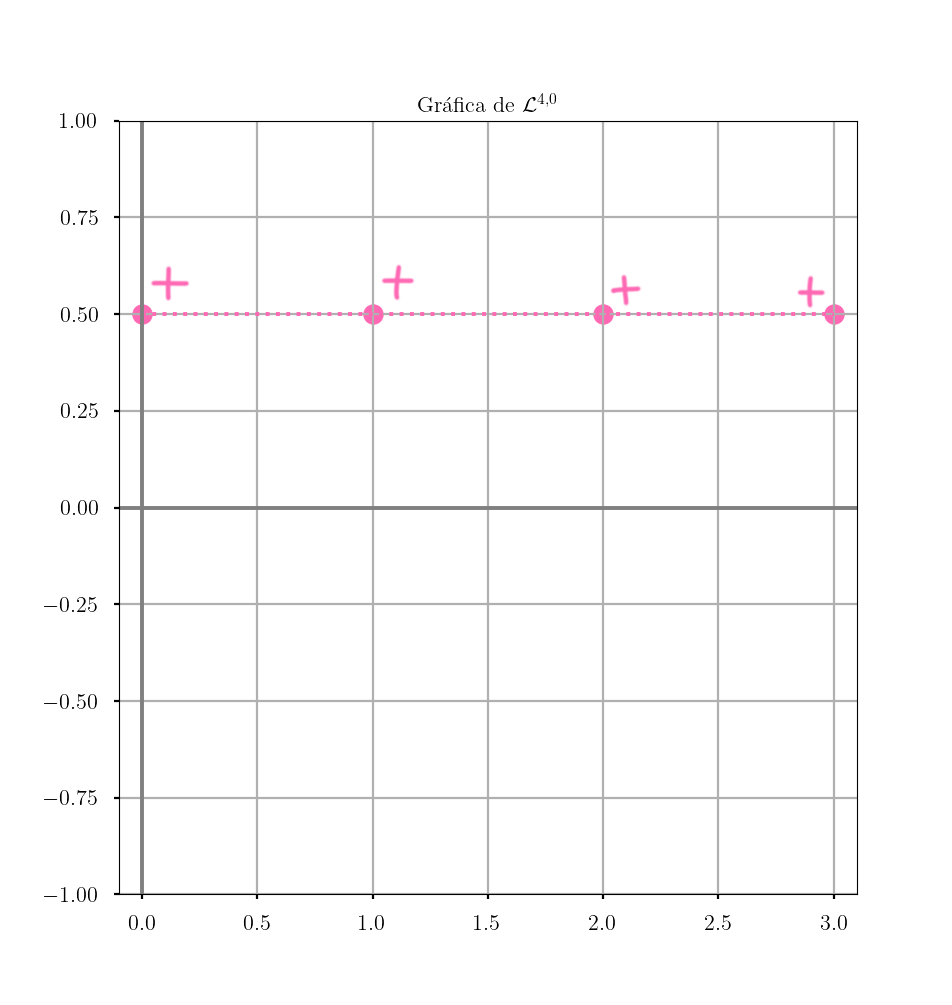
\includegraphics[scale=0.3]{oscil1}
\end{figure}
\end{minipage} \hfill
\begin{minipage}{0.45\textwidth}

1.- Por definición,

\[
\cali{L}^{4,0} = \left(
\frac{1}{2}, \frac{1}{2}, \frac{1}{2}, \frac{1}{2}
\right).
\]
\end{minipage}


\begin{minipage}{0.5\textwidth}
2.- La señal $\cali{L}^{4,1} \in \IR^{4}$ es un polinomio discreto de
dimensión 4 y grado 1 que se obtiene exigiendo las
siguientes condiciones

\[
\langle \cali{L}^{4,1} , \cali{L}^{4,0} \rangle=0
\hspace{0.2cm} \text{y} \hspace{0.2cm}
\langle \cali{L}^{4,1} , \cali{L}^{4,1} \rangle=1;
\]

esta primera condición se refleja en que 
las alturas de los puntos de la gráfica de 
$\cali{L}^{4,1}$ deben sumar cero;
esto implica un cambio de signo (y sólo uno,
pues el polinomio es lineal).

\end{minipage} \hfill
\begin{minipage}{0.45\textwidth}
\begin{figure}[H]
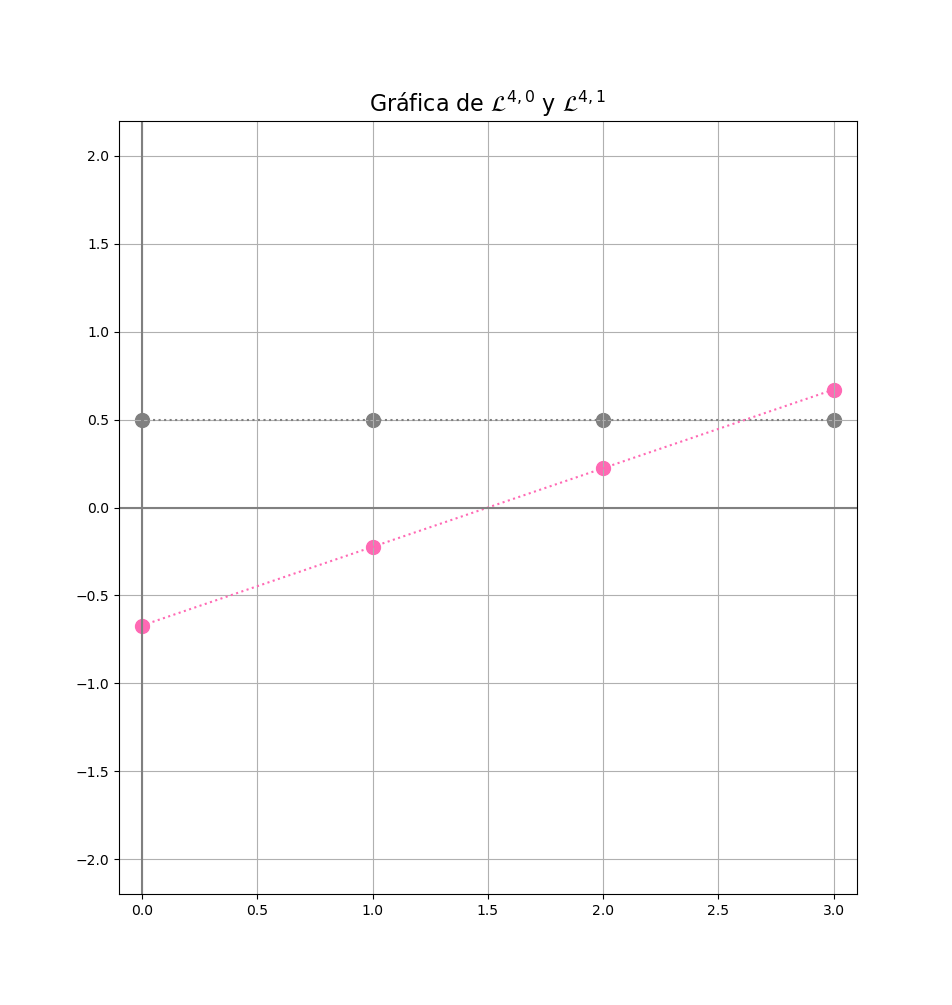
\includegraphics[scale=0.3]{oscil2}
\end{figure}
\end{minipage}

3.- Las condiciones de la definición
de $\cali{L}^{4,2} \in \IR^{4}$ son

\[
\langle \cali{L}^{4,2} , \cali{L}^{4,0} \rangle=0,
\hspace{0.2cm}
\langle \cali{L}^{4,2} , \cali{L}^{4,1} \rangle=0,
\hspace{0.2cm} \text{y} \hspace{0.2cm}
\langle \cali{L}^{4,2} , \cali{L}^{4,2} \rangle=1;
\]
observe que si las entradas de 
$\cali{L}^{4,2}$ fuesen todas positivas o todas negativas,
entonces no se tendría la ortogonalidad
con la señal constante $\cali{L}^{4,0}$. 

}
\begin{figure}[H]
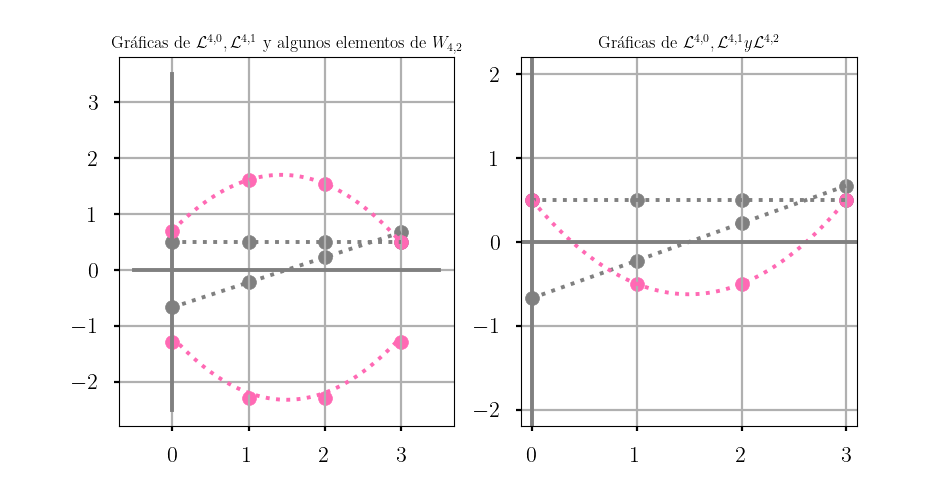
\includegraphics[scale=0.3]{oscil3}
\end{figure}

4.- 
\begin{figure}[H]
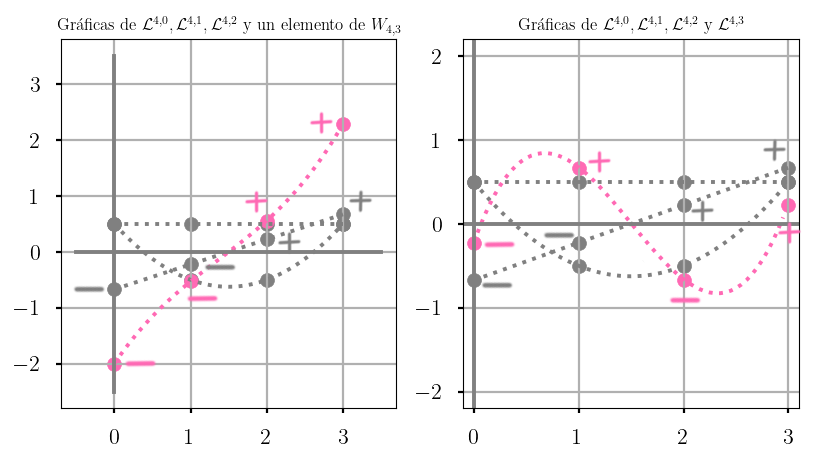
\includegraphics[scale=0.3]{oscil4}
\end{figure}